% !TEX root = ../thesis-example.tex
%
\chapter{Notation}
\label{ch:notation}

\cleanchapterquote{(...)building a musical instrument becomes indistinguishable from designing a music-theoretical framework; the musical instrument is a theory of music (...)}{Thor Magnusson}{Sonic Writing (2019)}

\cleanchapterquote{Tu sais comment je me suis adapté à ce problème de la radio dans l’environnement : comme les peuplades primitives se sont adaptées aux animaux qui les effrayaient et qui constituaient probablement, comme tu dis, des intrusions. Ils les ont dessinés sur les murs de leurs cavernes; et donc j’ai simplement composé une pièce avec des radios. À présent, à chaque fois que j’entends des radios – même une seule, pas forcément une douzaine en même temps, au moins, comme tu as dû l'entendre à la plage – je pense : ``Tiens, ils jouent ma pièce''.}{John Cage}{John Cage / Morton Feldman. \\ Radio Happenings 1966 \cite{cage_radio_2015}}

% This article presents “John”, an open-source software designed to help collective free improvisation. It provides generated screen-scores running on distributed, reactive web-browsers. The musicians can then concurrently edit the scores in their own browser. John is used by ONE, a septet playing improvised electro-acoustic music with digital musical instruments (DMI). One of the original features of John is that its design takes care of leaving the
% musician's attention as free as possible.
% Firstly, a quick review of the context of screen-based
% scores will help situate this research in the history of contemporary music notation. Then I will trace back how improvisation sessions led to John's particular “notational perspective”. A brief description of the software will precede a discussion about the various aspects guiding its design.

La citation de Cage\footnote{You know how I adjusted to that problem of the radio in the environment : very much as the primitive people adjusted to the animals which frightened them, and which probably, as you say, were intrusions. The drew pictures of them on their caves and so I simply made a piece using radios. Now, whenever I hear radios — even a single radio, not just twelve at a time as you must have heard on the beach, at least — I think : `Well, they're just playing my piece'.}

\noindent Dans ce dernier chapitre, j'aborde la question de la notation musicale, dont j'ai déjà évoqué les problèmes qu'elle posait dans le cas des musiques électroacoustiques au chapitre \ref{ch:ephemeral}. En particulier, j'y présente ``John, le semi-conducteur'', un logiciel de partition sur écran développé pour la pratique collective de l'improvisation libre électroacoustique avec l'ensemble \textit{ONE}, et les motivations qui ont conduit à ce développement.\\
\indent Au préalable, présenterai un état de l'art des partitions sur écran, ainsi que des considérations concernant la question de l'écriture musicale avec les \glspl{DMI}.

%%%%%%%%%%%%%%%%%%%%%%%%%%%%%%%%%%%%%%%%%
\section{Notes sur la partition}

\subsection{Du geste vers le son et vice versa}

\noindent La partition est généralement conçue comme un document permettant aux compositeurs de noter une œuvre musicale et de la transmettre à un instrumentiste en vue de son interprétation. Dans les partitions classiques de la notation musicale occidentale, la partition procède essentiellement de manière \textit{descriptive} en indiquant ce à quoi doit ressembler le résultat musical, par exemple la hauteur et la durée des notes. Avec la prise en compte croissante du timbre dans la notation musicale au cours des \siecle{19} et \siecle{20}~siècles, les partitions ont progressivement utilisé des annotations \textit{prescriptives} décrivant non plus le résultat sonore mais les actions à produire\footnote{L'exemple le plus manifeste de partition prescriptive étant probablement la pièce ``Imaginary landscape No 4'' de John Cage, où l'utilisation de radio rend impossible la description du résultat musical \textit{a priori}, tandis que les gestes de changement de gain et de fréquence sont précisément notés. Pour une étude plus approndie sur la notation du geste, voire notamment \cite{kojs_notating_2011}.}, à l'aide d'indications telles que ``\textit{con legno}'', ``\textit{sul ponticello}'' ou des symboles et explications ad-hoc\footnote{Eric Maestri propose les termes ``phonographique'' et ``ergographique'' pour décrire ceux deux aspects.} (cf. figure todo).

\noindent Dans le cas de l'utilisation de \glspl{DMI} ayant la capacité à produire des sons sans qu'il y ait nécessairement ``geste d'excitation'' (selon la terminologie de Cadoz) préalable, la partition peut servir à noter des ``gestes accompagnateurs''.\\
\indent Par exemple, dans la performance audiovisuelle FIB\_R, le cheminement vers la partition a été d'abord de construire un instrument, puis de jouer de cet instrument jusqu'à l'élaboration de formes musicales intéressantes. Mais à un certain moment, ce que l'on souhaitait ne correspondait plus à quelque chose d'explicitement jouable, car la précision rythmique désirée dépassait ce qu'il nous était possible d'atteindre avec les interfaces et l'algorithme de jeu utilisés. La machine laisse en effet la possibilité de créer des mouvements enregistrés dont la précision et la vitesse dépassent celles possibles pour un être humain. Il est intéressant, sur le plan artistique, d'explorer les zones à la limite des possibilités du corps, quand il reste envisageable pour le public de se projeter dans ces mouvements, tout en étant emmené dans une zone monstrueuse qui remet le corps en question.\\
\indent Nous avons donc fait le choix de séquencer intégralement la séquence, qui est techniquement ``jouée'' par la machine\footnote{Ce n'est pas un enregistrement audiovisuel pour autant, c'est bien le ``geste'' qui est pré-programmé et le résultat change à performance en fonction des paramètres de jeu des algorithmes.}. 
Par ailleurs, penser le geste indépendemment de sa capacité à être capté par la machine laissait la possibilité d'utiliser des gestes plus libres et plus en phase, musicalement, avec ce que nous souhaitions, sans nécessairement qu'ils suivent les détails micro-temporels.\\
\indent Il y a donc eu un renversement, entre des gestes qui servaient au début à produire des sons, pour arriver à une composition écrite et séquencée\footnote{La séquence musicale étant très rythmique, nous avons adopté une notation s'apparentant à celle de la percussion, dans laquelle chaque note désigne un type de geste particulier.} (cf. figures \ref{fig:notation:FIBR-chat2-Elle} et \ref{fig:notation:FIBR-chat2-Lui}), dont nous jouons les gestes de manière synchronisée.



%-------------------------- Figure : FIB_R Lui+Elle ----------------------------------
% \begin{figure}[!htbp]
% 	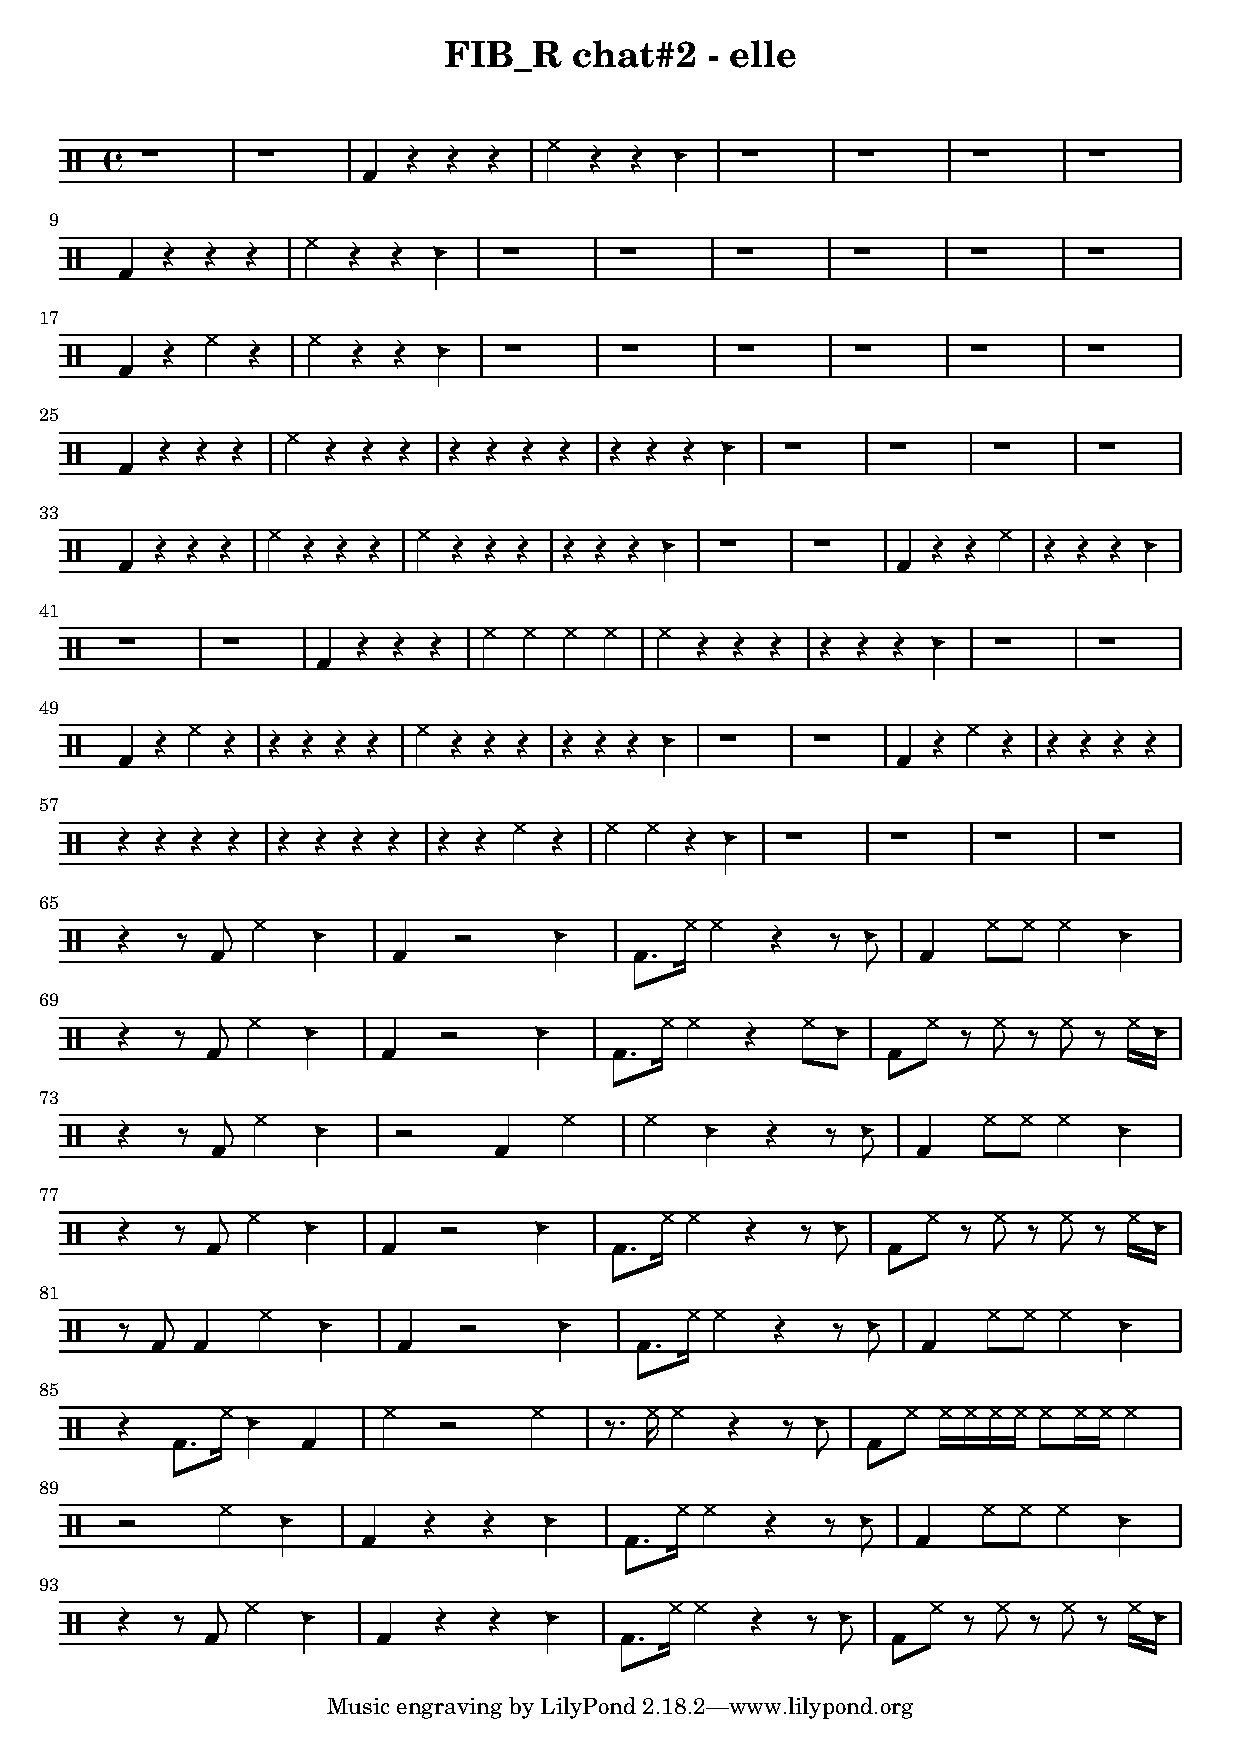
\includegraphics[width=\textwidth]{gfx/notation/FIBR-Chat2-Elle.pdf}
% 	\caption{Partition gestuelle pour la partie II de FIB\_R, Elle}
% 	\label{fig:notation:FIBR-chat2-Elle}
% \end{figure}

% \begin{figure}[!htbp]
% 	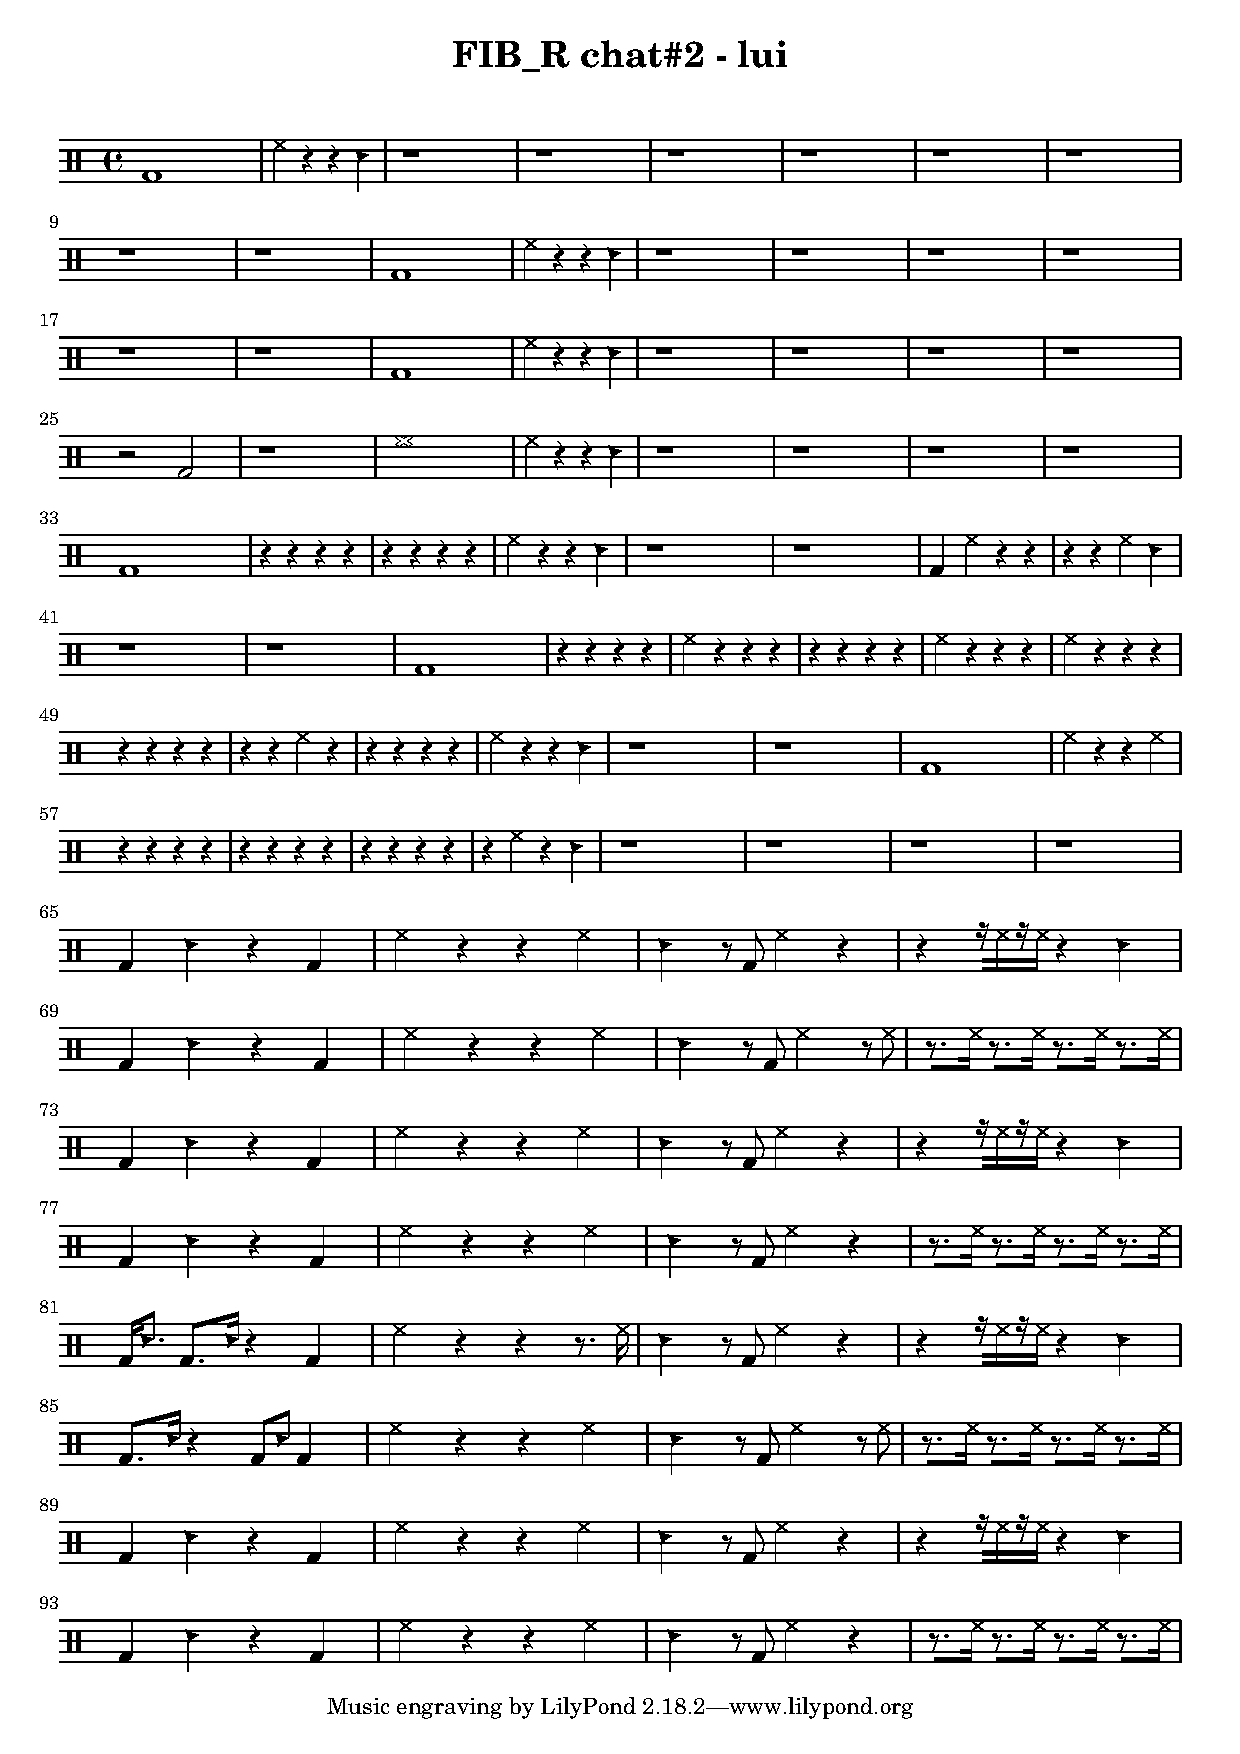
\includegraphics[width=\textwidth]{gfx/notation/FIBR-Chat2-Lui.pdf}
% 	\caption{Partition gestuelle pour la partie II de FIB\_R, Lui}
% 	\label{fig:notation:FIBR-chat2-Lui}
% \end{figure}

%------------ Figure : filigramophone et xypre HP -----------
\begin{figure}[!htbp]
	\captionsetup{format=plain}%
	\centering
	\begin{minipage}[t]{0.48\textwidth}
		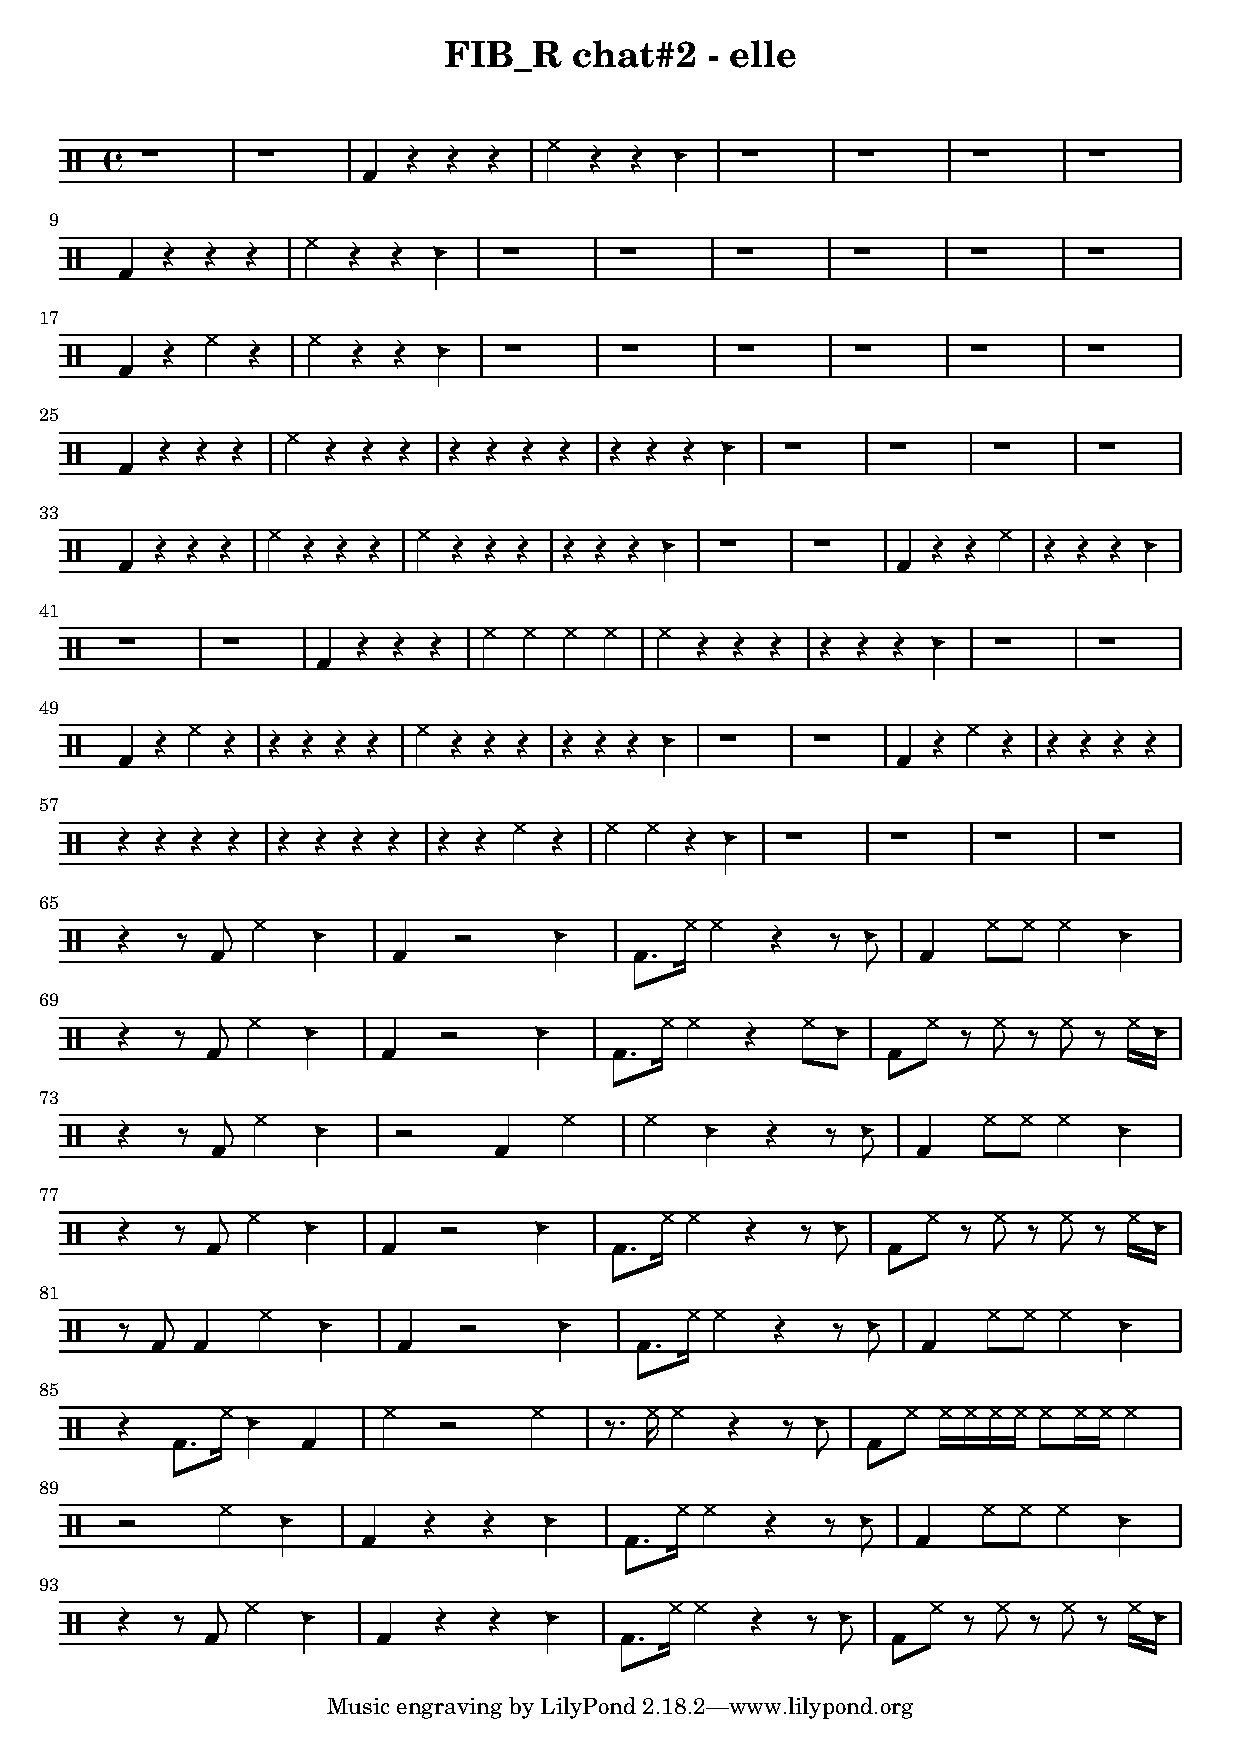
\includegraphics[width=\linewidth]{gfx/notation/FIBR-Chat2-Elle.pdf}
		\caption{Partition gestuelle pour la partie II de FIB\_R, Lui}
		\label{fig:notation:FIBR-chat2-Elle}
	\end{minipage}
	\hspace{.02\linewidth}
	\begin{minipage}[t]{0.48\textwidth}
	    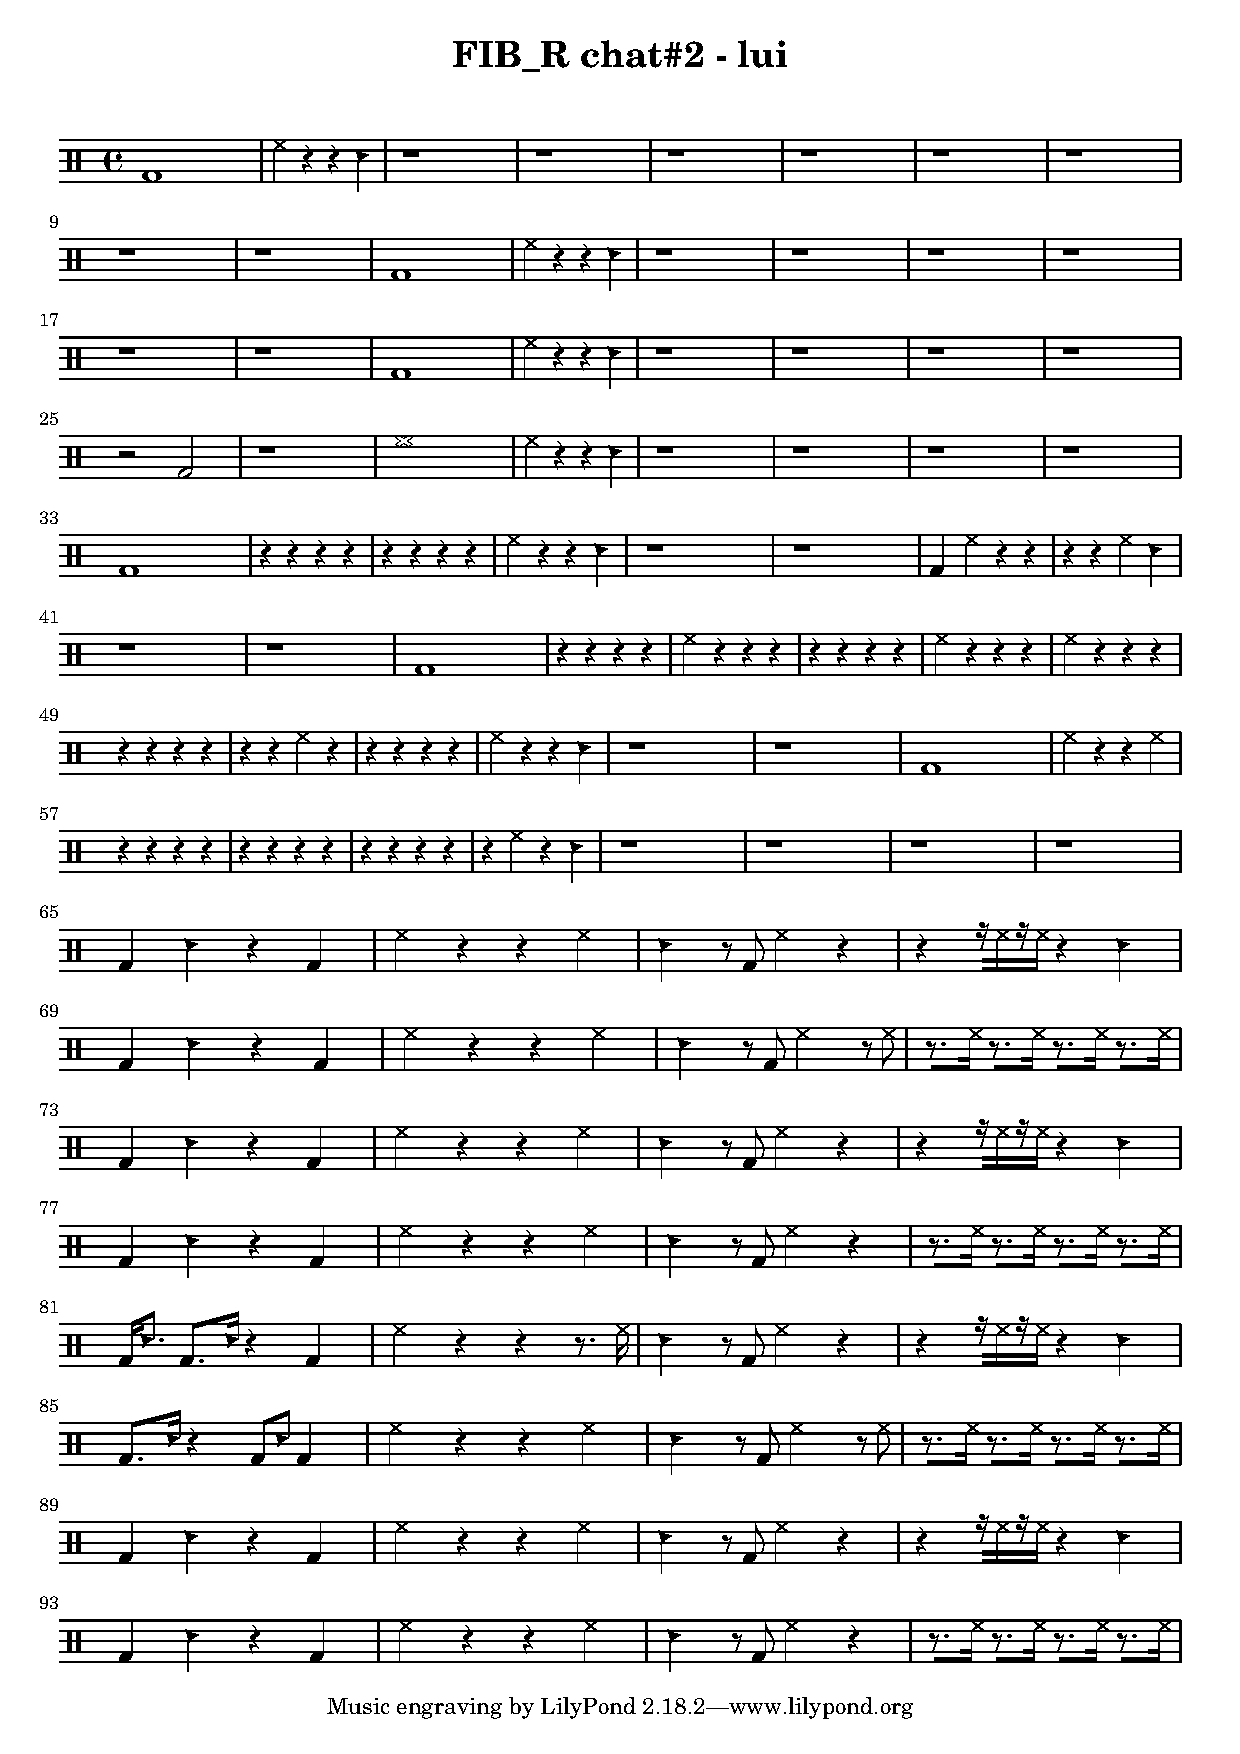
\includegraphics[width=\linewidth]{gfx/notation/FIBR-Chat2-Lui.pdf}
		\caption{Partition gestuelle pour la partie II de FIB\_R, Lui}
		\label{fig:notation:FIBR-chat2-Lui}
	\end{minipage}
\end{figure}
%------------ Figure : filigramophone et xypre HP -----------

extension d'impressions, intension d'expressions
%--------------------------------------------------------------------
\subsection{Des partitions traditionnelles aux partitions graphiques}

\noindent La partition est généralement considérée comme un document permettant au compositeur de transmettre une œuvre musicale à un interprète. Elle décrit le résultat sonore attendu et/ou prescrit les gestes à effectuer\footnote{Eric Maestri propose les termes ``phonographique'' et ``ergographique'' pour décrire ceux deux aspects.}. Elle sert ainsi de moyen mnémonique pour garder une trace de ce qui est indépendant du contexte de la performance\footnote{En considérant ici que l'interprétation fait partie du contextuel.} et qui est souvent assimilé à l'œuvre elle-même dans la tradition musicale occidentale.\\
\indent La partition possède cependant beaucoup d'autres fonctions. Elle permet notamment de transposer la temporalité musicale en une spatialité visuelle, permettant au compositeur d'agencer des éléments musicaux ``hors du temps'' afin de produire des pièces qui ne pourraient être conçues sans ce support visuel\footnote{Un exemple notoire est le rondeau ``Ma fin est mon commencement'' (\siecle{14}~siècle) de Machaut, dans lequel les deux voix sont rétrogrades l'une à l'autre.}.\\
\indent Si le système de notation occidental inventé par Guido d'Arezzo au \siecle{11}siècle n'a cessé d'évoluer, s'enrichissant de nouveaux symboles et de nouvelles techniques jusqu'au début du \siecle{20}~siècle, les révolutions technologiques et culturelles qui ont suivi ont bouleversé à la fois les moyens de production et le champ de l'expression musicale, désormais étendu au bruit et au spectre sonore entier.\\
\indent On peut noter l'essor de ce qu'on appelle les ``partitions graphiques''\footnote{... c'est-à-dire l'utilisation de signes graphiques autres que les symboles habituels de la notation conventionnelle des notes sur une portée.} au milieu du \siecle{20}~siècle, qui reflète cette évolution musicale pour laquelle la notation traditionnelle est insuffisante.  Pour des raisons qui peuvent sembler opposées, la partition graphique a contribué à repousser à la fois les limites de ce qu'il était possible de ``fixer'' dans une composition, en la spécifiant intégralement sur un système de synthèse, et les limites de ce qu'il était concevable de laisser sujet variations, c'est à dire la part confiée à l'interprétation du musicien.  Les partitions de \textit{Mycene Alpha} de Iannis Xenakis et de \textit{December 1952} de Earle Brown soulignent ces deux directions (cf. Figure \ref{fig:notation:brown-xenakis}).

%-------------------------- Figure : Brown-Xenakis ----------------------------------
\begin{figure}[!htbp]
	\captionsetup{format=plain}
	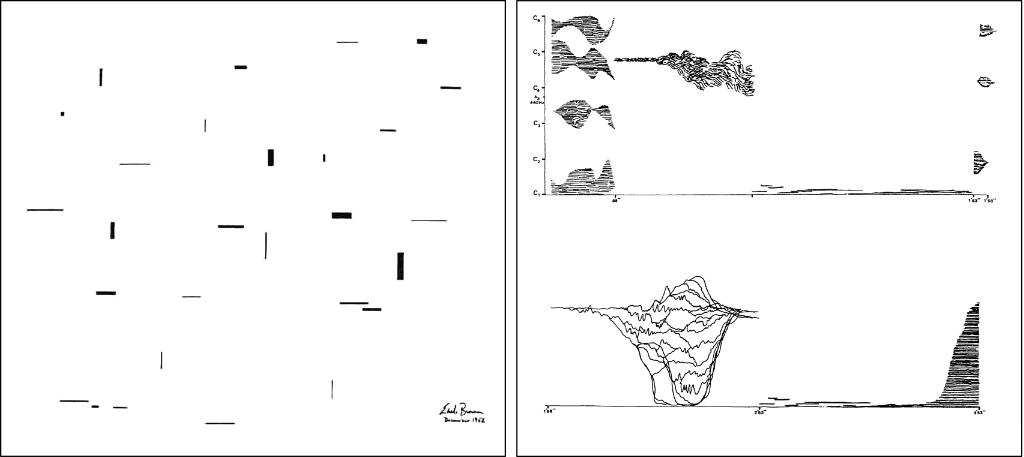
\includegraphics[width=\textwidth]{gfx/notation/Brown-Xenakis-Paysage.png}
	\caption{Extraits des partitions de \textit{December 1952} de Earle Brown (à gauche) et \textit{Mycène Alpha} de Iannis Xénakis (à droite)}
	\label{fig:notation:brown-xenakis}
\end{figure}

\noindent Cette opposition apparente entre une œuvre totalement figée et une œuvre totalement sujette à la sensibilité des interprètes semble plutôt le résultat d'approches complémentaires visant à explorer les nouveaux domaines sonores et musicaux, tant dans leurs manifestations que dans leurs potentialités, réifiées ou fantasmées.\\

%-------------------------------------------------------------------------
\subsection{Œuvres ouvertes et intension}

\noindent Parallèlement à cette part laissée à la sensibilité de l'interprète, le \textit{déroulement} de l'œuvre peut être sujet à variations. Si les partitions classiques se présentent généralement comme une description/prescription qui décrit le déroulement de la performance de manière linéaire et chronologique, les œuvres dites ``ouvertes''\footnote{Pour une présentation plus générale du concept d'œuvre ouverte, voir \cite{eco_oeuvre_2015}} fournissent aux musiciens des ``règles du jeu'' plutôt que qu'une image résultant du jeu de ces règles. L'œuvre ouverte peut intégrer des processus génératifs dont les résultats varient à chaque performance. 
\indent Jean-Louis Giavitto, dans \cite{giavitto_du_2014}, nomme ces deux types de partitions ``intensionelles'' et ``extensionnelles'' en référence à la formulation d'ensembles en mathématique, soit ``extensive'', c'est à dire définie par la liste explicite des valeurs de cet ensemble, soit ``intensive'', c'est à dire en les définissant par une propriété générative.

\subsection{Comprovisation}

\indent Dans ce continuum de possibilités entre œuvre fixe et improvisation libre, que Richard Dudas appelle \iquote{comprovisation} dans \cite{dudas_comprovisation:_2010}, différentes ``perspectives notationnelles''\footnote{j'emprunte ici cette expression à Baghwati \cite{bhagwati_notational_2013}} peuvent être envisagées. Les différentes finalités de la représentation musicale jusqu'alors intégrées dans la partition traditionnelle gagnent en indépendance et prennent une importance variable, s'adaptant aux contextes de l'œuvre musicale et de l'interprétation. La partition définit le terrain de jeu, qui n'est pas nécessairement linéaire et qui, notamment grâce à la possibilité de produire des images animées en temps réel, peut se reconfigurer dynamiquement durant le temps de la performance.


%-----------------------------------------------------------------------------
\subsection{Partitions sur écran}

\noindent La disponibilité croissante des appareils numériques a conduit au développement d'un certain nombre d'applications destinées à la création de partitions à l'écran. Comme le note Lindsay Vickery dans \cite{vickery_limitations_2014} : \iquote{Ces développements suggèrent une tendance, en particulier chez les jeunes compositeurs dont la pratique s'est développée exclusivement sur ordinateur, de passer logiquement à l'étape de présenter des matériaux notationnels à l'écran.}\\
\indent Cat Hope résume les principales caractéristiques offertes par ce nouveau média dans les termes suivants \cite{hope_screen_2011}: \textit{les capacités de défilement, de permutation, de transformation, de génération et de mise en réseau du support numérique}.\\
\indent L'utilisation de l'infographie pour la représentation musicale semble être un médium de choix pour enrichir les possibilités d'écriture de partitions graphiques. En particulier, la fluidité d'adaptation du support virtuel permet d'envisager de multiples ``vues'' d'une même partition selon les contextes auxquels elle est destinée. Ainsi, la composition, la performance ou l'analyse d'une œuvre musicale ne nécessitent pas nécessairement les mêmes représentations. En termes d'interprétation musicale, on peut ajouter une distinction entre l'interprétation d'une partition par un humain et une machine, ces deux types d'\textit{interprètes}\footnote{En informatique, on appelle ``interprète'' un outil ayant pour tâche d'analyser, de traduire et d'exécuter les programmes écrits dans un langage informatique.} ayant des capacités relativement différentes.\\
\indent De la même manière que les technologies numériques ont atomisé l'instrument de musique en découplant ses différentes composantes (contrôleur gestuel, cartographie, synthèse, etc. devenant modulaire), elles ont également atomisé la partition en ses différentes fonctions, de support pour la composition, la performance ou l'analyse. Il est alors nécessaire de préciser quel cas d'utilisation est en jeu et Cat Hope définit à cet effet le terme ``partition sur écran'' (\textit{screen-score}) \cite{hope_screen_2011} comme le medium présenté aux musiciens pour une performance: \iquote{Les partitions sur écran sont des compositions musicales écrites, conçues pour être interprétées ; elles ne doivent pas être confondues avec des représentations visuelles de la musique ou l'interprétation musicale des arts visuels.}\\
\indent Le concept de ``partition sur écran'' a été étudié par plusieurs chercheurs, compositeurs et musicologues (voir Winkler \cite{winkler_real-time_2004}, Clay \cite{adams_inventing_2008} ou Lee \cite{lee_real-time_2012}), qui ont discuté des avantages et des inconvénients de l'utilisation des technologies numériques pour la représentation musicale, tant dans ses aspects techniques que dans ses conséquences musicologiques. Lindsay Vickery propose par exemple une revue très détaillée dans \cite{vickery_limitations_2014}, des latences critiques permettant à un instrumentiste de lire en temps réel le matériel musical affiché et donne des conseils sur ce à quoi le compositeur doit faire attention lorsqu'il compose avec ce support.\\
\indent Ces études offrent des descriptions pertinentes et précieuses pour le compositeur qui souhaite utiliser des partition sur écran. Cependant, il semble qu'elles puissent être complétées par une approche de la partition différente de celles envisagées dans la plupart de la littérature sur le sujet, où le point de vue est souvent celui du compositeur. La conception d'un système de partition à écran est donc polarisée par l'importance centrale de la partition, elle-même considérée comme une condition préalable à l'exécution musicale, situation qui reflète également une forte tradition de la musique classique occidentale \footnote{Une exception notable est la contribution de Georg Hajdu \cite{hajdu_disposable_2016} qui propose le concept de ``musique jetable'' pour qualifier les formes musicales \iquote{qui reposent dans une moindre mesure sur des partitions entièrement notées, telles que la ``comprovisation'' ou la performance sur laptop}\footnote{\iquote{that rely on a lesser degree on fully notated scores, such as ``comprovisation'' or laptop performance}}. Cependant, même lorsqu'elle est ``jetable'', la partition occupe ici encore une position préalable à la performance et sur laquelle l'attention reste focalisée, à la différance de l'approche proposée avec ``John''.}.\\
\todo{déplacer ce dernier paragraphe dans la section suivante ?}
\indent Dans le cas des performances de ONE (Figure \ref{fig:notation:one-fullband}), qui sont basées sur une pratique d'improvisation libre sans composition préalable, la focale est déplacée du côté de l'instrumentiste. L'élément central n'est pas la partition mais l'écoute et la compréhension du son et des autres musiciens. La partition (s'il est encore possible de l'appeler ainsi) émerge souvent après les séances d'improvisation et sa présence ne doit pas se faire au détriment de l'attention mutuelle. Dans cette perspective, il est possible d'envisager que le musicien adapte lui-même la représentation musicale à ses propres besoins, en fonction des parties qu'il doit jouer, de ses préférences personnelles, des différents mouvements de la partition, etc.\\
\indent Dans le cas particulier où les instruments sont numériques et programmables, l'utilisation d'un système de partition en réseau offre également la possibilité de déléguer certains paramètres de l'instrument à un contrôle externe pris en charge par la partition. Dans une situation d'improvisation, la négociation entre ce contrôle automatisé et le choix du musicien implique une médiation que j'évoquerai dans la section \ref{sec:notation:score_for_humans_and_machines}.

%----------------------------------------------------------------------------------------------------------
\section{Improvisation dans ONE – genèse d'une notation}

\subsection{Présentation de ONE}

\noindent Les sept musiciens de l'ensemble ONE (cf. figure \ref{fig:notation:one-fullband}) sont tous profondément impliqués dans le domaine de l'informatique musicale avec des spécialités diverses dans les domaines de la pratique instrumentale, de la composition, de la facture instrumentale, de la recherche en sciences musicales et de l'éducation. Nous pratiquons tous des instruments de musique numériques dont nous avons conçu le logiciel\footnote{La plupart de ces \glspl{DMI} utilisent le logiciel Max pour le design de l'interaction, voire la synthèse.} et parfois aussi l'interface hardware, dans une certaine mesure.
A l'origine de notre collaboration, il n'y avait pas d'autre projet que celui de tenter l'expérience de jouer une ``musique de sons'' (todo : ref vers cette expression) avec cet instrumentarium numérique hétéroclite, sans grille, sans théorie musicale, sans accord préalable sur la forme et le contenu.\\

%-------------------------- Figure : ONE ----------------------------------
\begin{figure}[!htbp]
	\captionsetup{format=plain}%
	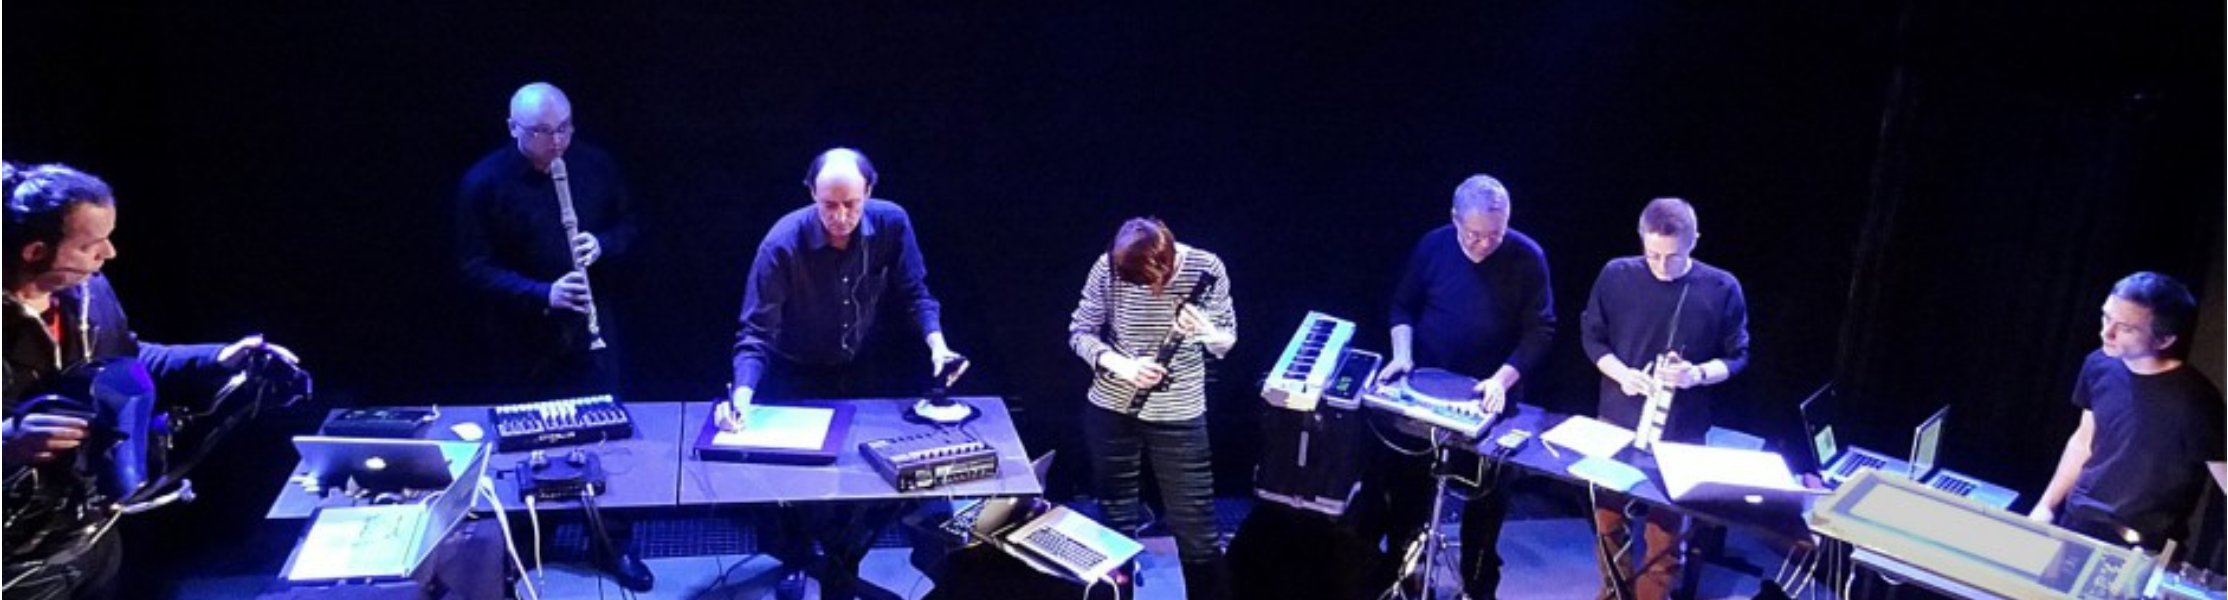
\includegraphics[width=\textwidth]{gfx/notation/ONE-fullBand.png}
	\caption[Les membres de ONE et leurs DMIs]{Les membre de ONE sur scène avec leurs \glspl{DMI}. De gauche à droite : Serge de Laubier au Méta-Instrument 3, Pierre Couprie à la flûte augmentée et interfaces MIDI, Hugues Genevois au Calliphone, Laurence Bouckaert au Karlax, György Kurtág Jr. au Handsonic, Jean Haury au Méta-Piano, Vincent Goudard au Filigramophone.}
	\label{fig:notation:one-fullband}
\end{figure}

\subsection{Improvisation libre et expérimentation}

\indent Plusieurs séances d'improvisation ont été l'opportunité de découvrir nos sons, nos styles de jeu, notre vocabulaire musical. Ces moments de répétition ont été avant tout l'occasion de performances anarchiques, guidées uniquement par le fil de notre écoute, de confrontation, de mélange, de collision, de superposition d'objets et d'espaces sonores, ainsi que de moments de discussion et de réglages de nos dispositifs de jeu.\\
\indent Ces sessions ont également fait l'objet d'exercices d'improvisation classiques : recherche de fusion timbrale et de contrepoints, passages fugués entre musiciens, accompagnement d'un soliste, travail sur les nuances pianissimo, ou improvisation ``dans le style'' d'une pièce connue. Finalement, les enregistrements audio nous ont permis de ré-écouter les improvisations parfois longues et ininterrompues pour en extraire des idées musicales intéressantes.\\

\subsection{Structurer le temps}

\indent La question de la structure globale d'un concert en mouvements musicaux est apparue durant la préparation de la première performance en public de ONE. L'absence d'une partition structurant la durée du concert nous a conduit à suivre un scénario narratif inspiré d'un roman de Jules Verne. Ainsi, le concert consistait en une série de chapitres, simplement identifiés par des intertitres tenant lieu de paysages sonores exotiques et imaginaires à explorer.\\
\indent Peu à peu, ces expériences ont donné lieu à l'émergence d'un vocabulaire musical plus atomique, représentant des atmosphères et des mouvements définis collectivement, que nous avons appelés ``karmas''\footnote{La relation avec ce concept indien est lointaine, mais elle comporte un sens séduisant qui fait écho à la façon dont nous les voyons dans la performance : l'ensemble des actions représentées par le karma influence l'avenir de l'individu. De même que l'interprétation musicale d'un \textit{karma} (tel que nous le définissons) est soumise aux actions des musiciens et tout accident, la bifurcation par rapport à la partition prévaudra sur l'évolution musicale plus que la partition elle-même.}. Les différents moments de jeu et de discussion nous ont amenés au développement d'autres objets conceptuels qui ont été en partie réalisés sous la forme d'un logiciel surnommé ``John, le semi-conducteur''\footnote{en anglais ``John, the semi-conductor'', ``conductor'' signifiant chef d'orchestre, ce subtil jeu de mot se perdant malheureusement dans sa traduction française...}.\\
\indent L'origine du développement de John est ainsi liée au désir de trouver un moyen de structurer le temps musical en différents mouvements dans la perspective de concerts librement improvisés d'une durée assez longue. 

\subsection{Stimuler la pratique en l'absence de chef}

Une autre motivation résidait dans la possibilité de générer des improvisations variées, afin de ne pas toujours répéter les mêmes textures et structures formelles telles que des séquences de cycles ascendants-descendants.\\
\indent De plus, nous cherchions des moyens de stimuler l'exploration de combinaisons et d'idées musicales inhabituelles qui nous poussent hors de notre zone de confort. La proposition de diviser mathématiquement le temps en séquences pour permettre à tous les ensembles possibles (solo, duo, trio, ... jusqu'au tutti), a été la première impulsion pour le développement d'un générateur de partition capable de produire automatiquement de telles distributions.\\
\indent Comme les opinions divergeaient au sein du groupe sur l'équilibre entre règles et absence de règles, un principe clé a permis de trouver un terrain d'entente : John est un ``semi-conducteur'', un ``sous-chef d'orchestre''. Cela signifie que les partitions créées avec John ne sont qu'une proposition, que chaque membre du groupe est libre de suivre ou non, selon le contexte musical qui ne prend véritablement forme qu'au moment même de la performance. L'écoute reste donc la règle essentielle du jeu, l'emportant sur un suivi aveugle de la partition. En particulier, sont laissés à l'appréciation de chaque musicien l'articulation entre les différentes parties de la partition, qu'elles soient tuilées ou disjointes, ou encore la décision de jouer quand il n'est pas censé le faire (ou inversement), etc.\\
\indent Ce principe a pour conséquence directe une épuration dans le design visuel de la partition, dont le but est de permettre à chaque musicien de se situer en un coup d'œil dans la partition, sans monopoliser son attention au détriment des autres musiciens et du son. Le but est donc très différent de celui poursuivi dans d'autres systèmes de notation musicale sur écran, comme ceux explorés dans des travaux impliquant du déchiffrage en direct de partition dynamique \cite{freeman_extreme_2008}.\\

\indent Ainsi, John permet la gestion collective du temps, que ce soit lors des répétitions, de la composition ou des performances, en fournissant un support de représentation partagé. Une brève description du logiciel pour en saisir les grandes lignes précédera une discussion sur les différents aspects liés à cette gestion de groupe.

%%%%%%%%%%%%%%%%%%%%%%%%%%%%%%%%%%%%%%%%%
\section{John, the semi-conductor}

\noindent John s'appuie sur une architecture client / serveur, dans laquelle chaque musicien visualise une interface client dans un navigateur web, sur laquelle il peut agir. Cette interface se compose de deux parties, un générateur de partition d'une part et une visualisation interactive de la partition d'autre part.
%-------------------------- Figure : John client interface ----------------------------------
\begin{figure}[!htbp]
	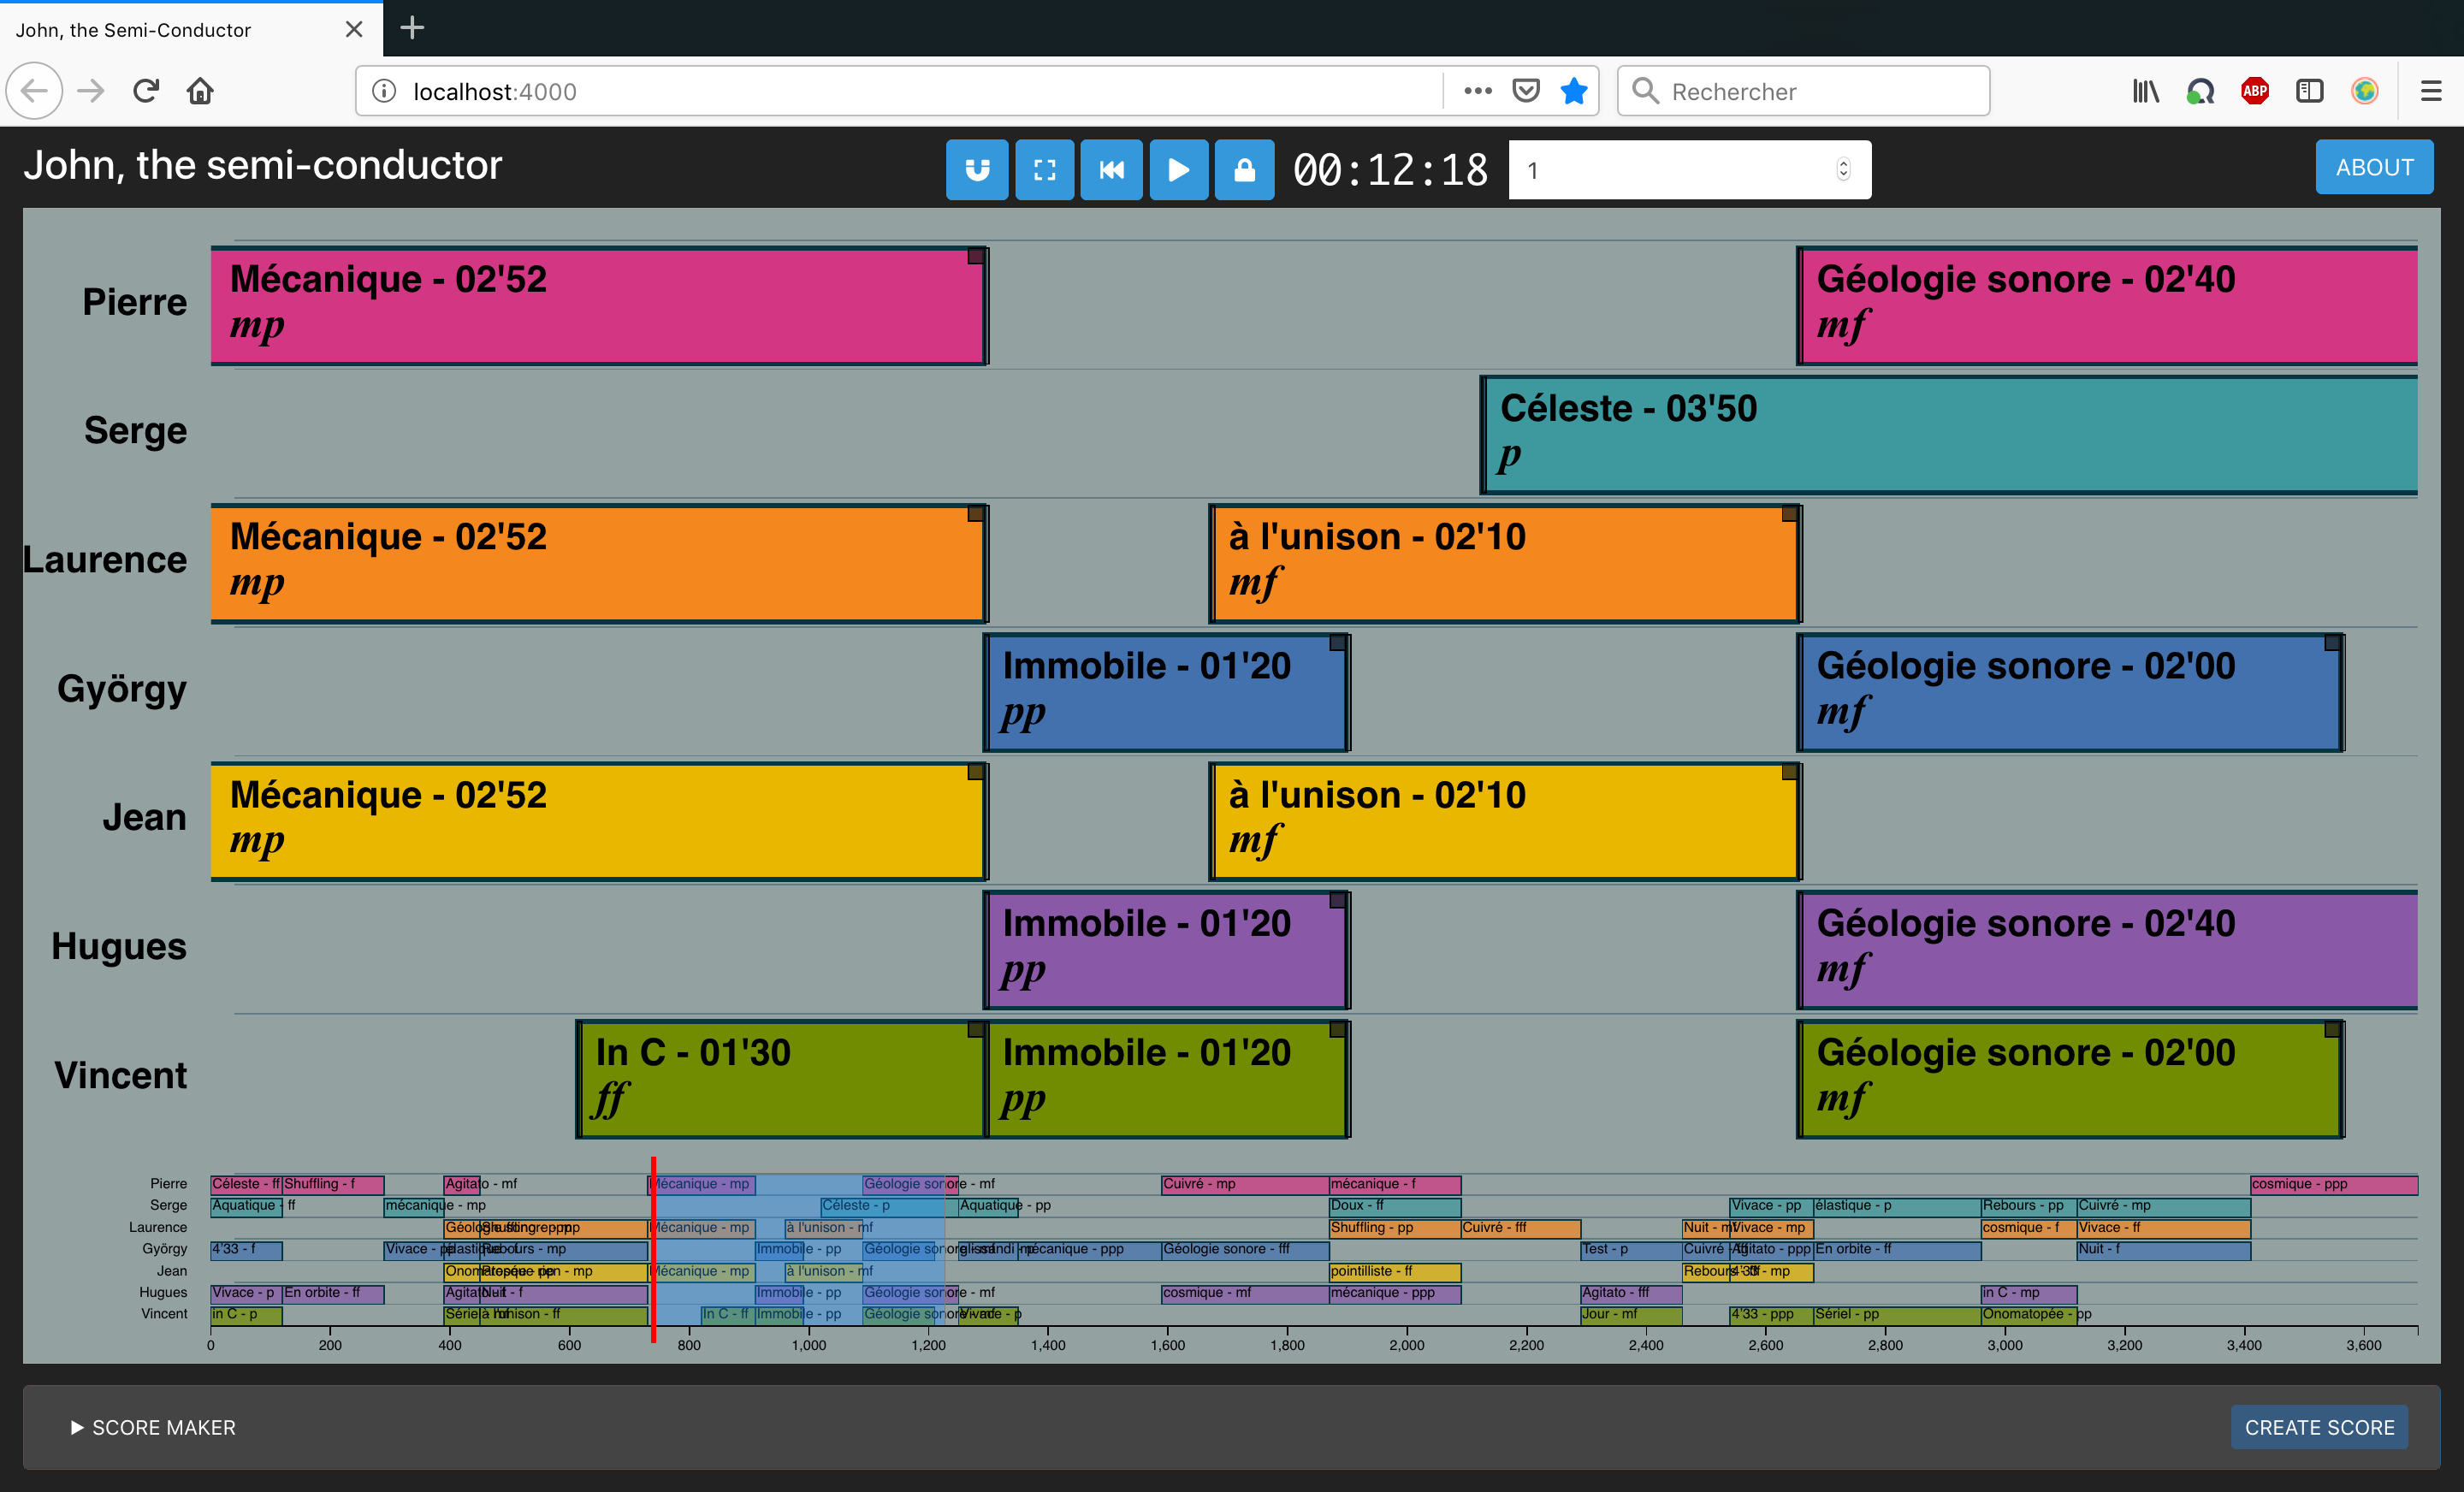
\includegraphics[width=\textwidth]{gfx/notation/John-snapshot.png}
	\caption{Snapshot of John's client interface running in a web-browser.}
	\label{fig:notation:john-snapshot}
\end{figure}

%----------------------------------------------------------------------------------------------------------
\subsection{Générateur de partitions}

\noindent Le générateur de partitions permet de créer très rapidement des propositions musicales en ne spécifiant que des contraintes globales :
\begin{itemize}[noitemsep]
\item la durée globale de la partition;
\item le nombre minimal et maximal de joueurs;
\item la durée minimale et maximale des blocs;
\item une liste de \textit{karmas} identifiant une ambiance musicale particulière, selon un vocabulaire défini en commun durant les séances d'improvisation;
\item une liste de nuances de \textit{pianississimo} à \textit{fortississimo}.
\end{itemize}

\noindent Une fois ces contraintes spécifiées, le générateur de partition produit une proposition aléatoire respectant ces conditions, composée d'une séquence de blocs temporels associant un karma et une nuance. Cette proposition peut ensuite être ajustée dans l'interface d'édition / visualisation.

%----------------------------------------------------------------------------------------------------------
\subsection{Visualisation interactive}

\noindent Cette interface représente des blocs sur disposés sur une abscisse chronologique. Elle se compose d'une \textit{vue globale} réduite d'une part, offrant une vue d'ensemble partagée de la partition dans son intégralité, et d'une \textit{vue locale} zoomable, située au-dessus de la \textit{vue globale}. Sur la \textit{vue globale} se trouve une tête de lecture commune et synchrone à tous les clients (en rouge sur la Figure \ref{fig:notation:john-snapshot}), ainsi qu'un empant temporel (en bleu sur la Figure \ref{fig:notation:john-snapshot}) définissant la durée affichée sur la \textit{vue locale}. Cet empant est défini individuellement par chaque musicien sur son client et varie généralement d'une dizaine de secondes à quelques minutes selon la granularité temporelle de la partition et la préférence de chacun.\\
\indent Tous les paramètres de contrôles sont accessibles dans l'ensemble des clients, permettant à chacun d'éditer la partition : générer une nouvelle instance, déplacer et modifier la durée des blocs et leur contenu (\textit{karma} et \textit{nuance}), démarrer la lecture, modifier la vitesse de lecture, déplacer la tête de lecture pour démarrer à un moment donné de la partition. Ces changements sont immédiatement appliqués à l'ensemble des autres clients de John.\\
\indent L'utilisateur peut également définir des paramètres locaux qui n'affecteront que son interface client : la visibilité des différentes pistes, la durée de sa \textit{vue locale} et la synchronisation (ou non) de sa vue locale au curseur de lecture, à l'aide du bouton ``link''.

%----------------------------------------------------------------------------------------------------------
\subsection{Implémentation}

\noindent Après une première version développée en Max\footnote{\url{https://cycling74.com}}, l'application a été portée en HTML5 réactif à l'aide de l'environnement Meteor\footnote{\url{http://meteor.com}}. Ceci permet l'édition collective sur toutes les plates-formes (y compris les plates-formes mobiles) connectées à un réseau local, via un simple navigateur web. La visualisation a été réalisée à l'aide de la bibliothèque D3.js\footnote{\url{https://d3js.org}}.\\
\indent Les partitions sont sauvegardées au format \gls{JSON} sous la forme d'une liste d'événements avec un identifiant unique, un index de piste, une temps de début, une durée et un certain nombre de propriétés telles que le karma et les nuances. Pendant la lecture, le temps et les événements de la paritition sont envoyés en tant que messages MP (cf. section \ref{sec:algorithms:MP}) sur le réseau.

%%%%%%%%%%%%%%%%%%%%%%%%%%%%%%%%%%%%%%%%%
\section{John en pratique}
%----------------------------------------------------------------------------------------------------------
\subsection{Composition générative}

\noindent Le générateur de partitions nous a fait gagner beaucoup de temps pendant les répétitions, en nous offrant immédiatement une structure musicale possible. Aussi arbitraire que soit cette structure, sa fonction principale est de stimuler la performance musicale via sa prescription la plus minimale : quand jouer (ou ne pas jouer). Ainsi, les propositions sont souvent testées telles quelles avant d'être ajustées collectivement en fonction de ce que les membres du groupe trouvent intéressant ou non. Il est alors possible de faire évoluer cette structure musicale, avec apparemment plus d'efficacité que si l'on partait de rien.

%----------------------------------------------------------------------------------------------------------
\subsection{Distribution de la participation}

\noindent Le fait que John propose explicitement une distribution du temps de jeu entre chaque musicien a conduit à des configuration d'ensemble que nous n'aurions pas nécessairement essayées, en particulier les ensembles réduits (solo et duo), chacun d'entre nous ayant tendance à jouer trop souvent pour laisser s'installer ces configurations minimales.\\
\indent De plus, avoir des moments de pause explicites permet de mieux anticiper ses entrées. En effet, les \glspl{DMI} ont souvent une dimension ``méta-instrumentale''\footnote{C'est-à-dire qu'il peut être totalement reconfiguré pendant la représentation pour offrir un tout autre ensemble de sons, de processus et de modes de jeu.}, et plus généralement ils exposent un grand nombre de paramètres. Ces moments de pause planifiés permettent de mieux gérer le temps dont dispose chaque instrumentiste pour configurer de telles reconfigurations de paramètres. (todo: expliquer un peu mieux la distinction entre paramètres accessibles immédiatement et paramètres moins accessibles)

%----------------------------------------------------------------------------------------------------------
\subsection{Synchronisation}

\noindent Dans une situation d'improvisation libre, la synchronisation entre les musiciens est entravée par l'absence de règles idiomatiques. En particulier, l'absence de pulsation ou de mesure rend cette synchronisation plus difficile encore quand le nombre de musicien augmente et prive souvent l'improvisation libre de transitions franches dans la pratique d'ensemble.

\indent Le chef d'orchestre, lorsqu'il y en a un, fournit des repères temporels précis, par la battue et d'éventuelles indications pour le jeu. Outre les questions éthiques posées par le rôle d'un leader d'un groupe d'improvisation, et analysées par Clément Canonne dans \cite{canonne_improvisation_2012}, confier la direction d'une improvisation à une personne\footnote{comme c'est le cas dans le \textit{Soundpainting} de Walter Thomson ou dans une composition comme ``Cobra'' de John Zorn} reste limité par le fait qu'elle ne peut agir que dans le présent, et que cela exige une attention quasi-permanente des musiciens envers le chef, au détriment de celle qu'ils peuvent porter à leurs pairs. A cet égard, la représentation offerte par John condense d'une certaine manière la partition et le chef d'orchestre dans un seul et même support visuel. Cette partition animée offre en effet des repères visuels qui indiquent la simultanéité de plusieurs événements musicaux, et son défilement sous la tête de lecture permet une synchronisation précise entre les musiciens lors des transitions.\\

%----------------------------------------------------------------------------------------------------------
\subsection{Support visuel pour des repères musicaux}

\noindent Malgré la disponibilité d'outils d'analyse\footnote{Tels que E-Analysis \cite{couprie_eanalysis:_2016} ou l'Acousmographe du \gls{GRM} \cite{favreau_lacousmographe_2010}.} et l'existence d'un certain vocabulaire pour décrire les objets sonores et musicaux dans la musique électroacoustique\footnote{en particulier les ``objets sonores'' de Pierre Schaeffer \cite{schaeffer_traite_1966}, les ``images-son'' de François Bayle \cite{bayle_musique_1993} ou encore les \gls{UST} du \gls{MIM} \cite{delalande_les_1996}.}, il n'existe aucune norme de notation prescriptive pour les \glspl{DMI}. L'absence d'un vocabulaire unanime, la singularité des instruments et la formidable palette sonore qu'ils offrent, ne facilitent pas l'exercice consistant à identifier et discuter ce qui vient d'être joué lors d'une longue séance d'improvisation (manquant de pouvoir parler ici de ``répétition''). Une partition minimale telle que celle proposée par John facilite cette identification et permet de retravailler des moments précis après une longue performance. La réduction que la notation symbolique opère sur le résultat sonore complexe d'une performance permet à chacun de se retrouver rapidement dans l'espace temporel d'une improvisation, plus rapidement du moins que si l'on devait se référer à l'enregistrement sonore.

%----------------------------------------------------------------------------------------------------------
\subsection{Une écologie de l'attention}

\noindent L'improvisation libre électroacoustique requiert une attention considérable des musiciens envers les autres musiciens, leur instrument et, de toute évidence, au son. À cet égard, les \gls{DMI} présentent souvent l'inconvénient supplémentaire, par rapport aux instruments acoustiques, de capter une partie de l'attention visuelle en raison de la présence fréquente d'un écran, de nombreux paramètres d'interaction et d'une interface parfois dépourvue de retours ou de repères tactiles qui permettraient d'y accéder sans avoir besoin de les regarder. De plus, les musiciens numériques préparent souvent leur instrumentarium juste avant la représentation\footnote{ce que Thor Magnusson et Kris Kiefer nomme ``pre-grammation'' dans \cite{kiefer_live_2019}} avec un ensemble choisi d'éléments musicaux \textit{ad hoc} (lorsqu'ils ne le codent pas en direct, comme c'est le cas dans le live-coding), ce qui complique encore la connaissance ``kinesthésique'' de l'ergonomie de l'instrument, sans aucune aide visuelle.\\
\indent La conception de ``John'' a été ainsi motivée par une économie de la charge cognitive des musiciens. Pouvoir en partie personnaliser son interface de visualisation ne signifie donc pas y ajouter davantage de données visuelles, mais plutôt n'afficher que ce qui est nécessaire, au profit de l'attention mutuelle.

%----------------------------------------------------------------------------------------------------------
\subsection{Partitions pour humains \emph{et} machines}
\label{sec:notation:score_for_humans_and_machines}

\noindent Pendant la lecture de la partition, le serveur envoie des données aux clients lorsque des événements commencent ou se terminent (cf. figure TODO). Ces informations peuvent être utilisées par l'instrument du musicien (si toutefois son \gls{DMI} est connecté au réseau). Mais, comme John n'est qu'un ``semi-conducteur'', ses messages peuvent tout aussi bien être soumis à l'approbation du musicien/client pour permettre une certaine flexibilité dans la façon dont le musicien adhère à la partition.\\
\indent Ainsi, il est possible d'imaginer qu'un \textit{karma} spécifique rappelle un pré-réglage correspondant dans l'instrument du musicien, correspondant à l'esprit de ce \textit{karma}. Mais si le musicien est encore en train de jouer le \textit{karma} précédent, il/elle ne voudra probablement pas que cette notification change automatiquement sa configuration avant d'avoir terminé la phrase musicale en cours. Cette ``évaluation paresseuse''\footnote{J'emprunte ici ce terme utilisée dans le domaine de la programmation récursive, qui consiste à évaluer une expression uniquement quand le résultat de cette expression devient nécessaire. Dans notre cas toutefois, c'est possiblement le musicien qui décide de cette évaluation.} rend l'utilisation de John un peu différente de celle des séquenceurs traditionnels.

%----------------------------------------------------------------------------------------------------------
\subsection{Montrer la partition ?}

\noindent Rendre lisible les interactions entre les musiciens dans les performances d'improvisation peut contribuer à l'appréciation globale de la performance par le public. Pourtant, avec les \glspl{DMI}, le découplage spatial et énergétique entre les gestes de l'instrumentiste et la localisation de l'énergie sonore (sur un haut-parleur possiblement distant) brouille cette lecture. Les systèmes de partition sur écran offre la possibilité de partager l'affichage de la partition avec le public plus facilement que ne le permettent les partitions imprimées et peuvent ainsi aider à cette lisibilité avec le risque, cependant, qu'elle ``entrave les aspects performatifs dramatiques de l'œuvre'' parmi d'autres raisons suggérées par Cat Hope dans \cite{hope_screen_2011}.\\
\indent Bien que la partition de John n'ait jamais été montrée directement au public pour cette raison particulière, elle a été utilisée pour contrôler des effets vidéo et de lumières\footnote{Il s'agissait par exemple d'éclairer les musiciens censés jouer, de modifier la teinte de la lumière en fonction des karmas, de projeter des ondes sonores agrégées comme traces de la partition, de synchroniser des vidéos, etc.}, à la fois des raisons scénographiques et pour aider l'écoute à la compréhension de la musique.

%%%%%%%%%%%%%%%%%%%%%%%%%%%%%%%%%%%%%%%%%
\section{Perspectives}

\noindent Les membres de ONE ont reconnu que John aidait le processus créatif. Cependant, il reste des questions ouvertes comme la synchronisation collective sur les passages rythmiques. En particulier, anticiper un processus dynamique n'est pas une tâche triviale et nécessiterait probablement des outils spécifiques à cette fin, telles que les animations proposées par Ryan Ross Smith dans \cite{smith_atomic_2015}.\\
\indent Le concept de vues \textit{locale} et \textit{globale} pourrait probablement être généralisé à d'autres paramètres partageables. Par exemple, pouvoir démarrer une lecture locale pour s'entraîner ou préparer son instrument par soi-même. De même, il serait utile de travailler sur une autre partition que celle chargée sur les autres clients. Cette désynchronisation soulève cependant des problèmes de conflits de versionnage, dont la prise en compte dépasse pour l'instant les possibilités offertes par John.\\
\indent Le portage de John sur une technologie web a été en partie motivé par la possibilité de futurs concerts impliquant un grand nombre de musiciens et dans lesquel chaque musicien pourrait voir sa partie avec un simple navigateur web. D'autres développements seront nécessaires pour pouvoir réaliser de telles performances, qui posent là-encore des questions d'ergonomie visuelle.
\indent Dans l'ensemble, les partitions informatisés laissent place à de nombreuses interactions possibles pendant la durée de la performance. Leur design pourrait probablement tirer partie du fait de les considérer comme un instrument collectif, dont chaque musicien, ceci incluant public et son écoute active, pourrait jouer.
